\chapter{Processore}

\section{Processore}

A partire dall’implementazione fornita di un processore operante secondo il modello IJVM, 
a)	si proceda all’analisi dell’architettura mediante simulazione e si approfondisca lo studio del suo funzionamento per due istruzioni a scelta, 
b)	si modifichi un codice operativo a scelta, documentando tutte le modifiche effettuate,
c)	(opzionale) si descriva il funzionamento del processore in merito alle istruzioni di input/output,
d)	(solo ove possibile) si sintetizzi il processore su FPGA.

\subsection{Architettura MIC-1}
Il processore MIC-1 è caratterizzato da un'architettura a stack, composta da due componenti principali: control unit e datapath.
Lo stack permette di memorizzare i diversi operandi necessari alle varie operazioni e si trova in memoria. Per poterlo utilizzare sono necessari due registri, lo \textit{Stack Pointer(SP)} (che punta sempre all'ultimo elemento inserito nello stack) e il \textit{Top Of Stack (TOS)} (il valore puntato). 

Di seguito viene mostrato uno schema dell'architettura generale.
\begin{figure}[H]
    \centering
    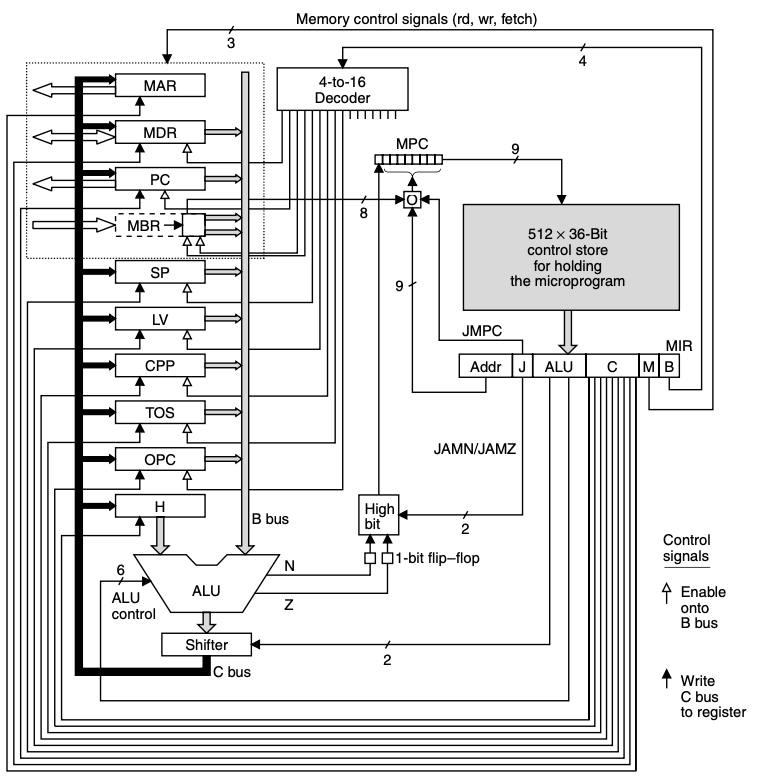
\includegraphics[width=16cm]{immagini/esercizio8/mic1_arch.png}
    \caption{Architettura MIC-1}
    \label{fig:mic1_arch}
\end{figure}

\subsubsection{Control Unit}
La \textit{control unit} stabilisce qual è la prossima microistruzione da prendere dalla ROM e, conoscendo il suo formato, si occupa di abilitare i segnali appropriati del datapath.
In particolare, il microprogramma è memorizzato nella ROM 512x36 chiamata Control Store, e per potervi accedere si utilizza il registro,\textit{ MPC (MicroProgram Counter)}. 
Ciascuna microistruzione (Control Word) è composta da 36 bit ed è strutturata come mostrato in figura:

\begin{figure}[H]
    \centering
    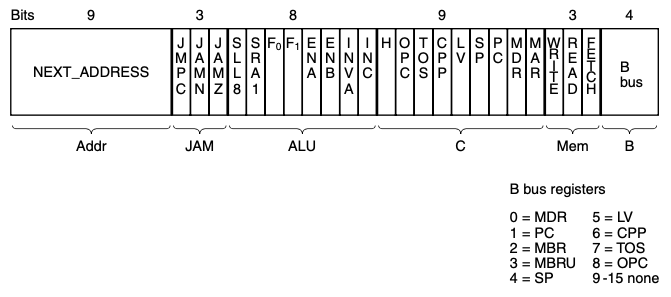
\includegraphics[width=16cm]{immagini/esercizio8/mic1_instr.png}
    \caption{Formato microistruzione del MIC-1}
    \label{fig:mic1_instr}
\end{figure}

Di seguito sono descritti i vari campi della Control Word:
\begin{itemize}
\item Addr: Indirizzo a 9 bit di una potenziale prossima microistruzione da inserire nel MPC. Questo indirizzo viene combinato con i segnali \textit{N} e \textit{Z} (in uscita dall'ALU) e \textit{JAMN}, \textit{JAPZ} e \textit{JMPC} per effettuare eventuali salti. 
\item JAM: I tre bit della sezione JAM specificano eventuali salti  che alterano il flusso lineare dell'indirizzamento in memoria;
\item ALU: Controllo dell'ALU e dello shifter con cui specificare le operazioni da svolgere. In particolare, l'ALU è controllata da 6 bit ed è alimentata dal bus B e dal registro H, mentre lo \textit{shifter} viene controllato da 2 bit.
\item C: Controlla quali registri vengono scritti dal bus C. Il bus C è in lettura e viene controllato esplicitamente da 9 bit. Questa scelta da la possibilità di scrivere i valori in più registri contemporaneamente.
\item Mem: Tre bit per controllare le operazioni di memoria. Pur avendo 2 coppie di registri MAR-MDR (che usano parole da 32 bit) e PC-MBR (che usano parole da 8 bit) sono necessari solo 3 bit poiché l'operazione di scrittura non ha senso per il \textit{Program Counter}.
\item B: Seleziona il registro connesso al bus B. Essendo un bus di scrittura, e quindi accessibile \textbf{solo} in mutua esclusione dai registri del \textit{datapath}, è conveniente effettuare una codifica dei segnali di abilitazione per rendere la memoria più piccola. In particolare, essendo 9 i registri che devono scrivere, è necessaria una codifica su 4 bit. Questa scelta comporta l'introduzione di un \textit{decoder} 4-16 nell'architettura.
\end{itemize}


\subsubsection{Datapath}
Il datapath è costituito da 9 registri, un ALU e uno \textit{shift register} controllati attraverso due bus separati: il bus B, necessario alla scrittura, e il bus C per la lettura.

L'ALU ha i seguenti ingressi:
\begin{itemize}
    \item A: collegato al registro H;
    \item B: collegato al bus B;
    \item Controlli: 6 segnali provenienti dall'unità di controllo;
\end{itemize}

Mentre fornisce le seguenti uscite:
\begin{itemize}
    \item N: bit alto se il risultato è negativo;
    \item Z: bit alto se il risultato è zero;
    \item OUT: risultato delle operazioni che viene messo in ingresso allo \textit{shift register};
\end{itemize}

\subsubsection{Interazione con la memoria}
Ci sono una serie di registri adibiti alla comunicazione con la memoria. Come detto in precedenza, sono controllati dai segnali MEM\_X presenti nelle micro-istruzioni. In particolare, si dividono in due coppie:
\begin{itemize}
    \item MAR-MDR: registri a 32 bit che servono a leggere e scrivere dalla memoria. In particolare, il MAR contiene l'indirizzo con cui avverrà la lettura/scrittura; mentre in MDR sarà presente il dato letto/scritto. Inoltre, la scrittura avviene in un colpo di clock ed è necessario fornire un segnali di abilitazione; invece la lettura avviene in due colpi di clock e non è necessario un'abilitazione;
    \item MBR-PC: registri a 8 bit da cui è possibile solo leggere byte dalla memoria. Per questo motivo, una microistruzione può portare più accessi in memoria;
\end{itemize}
\begin{figure}[H]
    \centering
    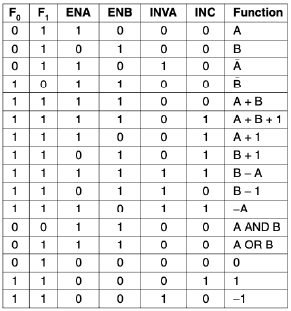
\includegraphics[width=10cm]{immagini/esercizio8/ALU.png}
    \caption{Tabella delle operazioni ALU}
    \label{fig:alu}
\end{figure}


\subsubsection{Analisi BIPUSH}
In questa sezione viene esaminata il codice operativo BIPUSH, analizzando le singole microistruzioni.

BIPUSH = 0x10:
\begin{enumerate}
\item SP = MAR = SP + 1 : in questa microistruzione viene incrementato lo stack pointer e il nuovo indirizzo viene caricato all'interno del MAR, in modo da specificare la locazione di memoria dove inserire il nuovo dato.
\item PC = PC + 1; fetch : questa microistruzione è presente in ogni codice operativo e serve a prepararsi per la prossima operazione.
\item MDR = TOS = MBR; wr; goto main : l'operando memorizzato nell'MBR viene inserito nel TOS che a sua volta viene inserito nel MDR. Successivamente, col segnale wr, viene abilitata la scrittura. 

\end{enumerate}
Ognuna delle microistruzioni viene rappresentata da una stringa di 36 bit, come descritto in precedenza, e nel caso della BIPUSH la prima è composta dai seguenti campi:
\begin{itemize}
    \item  ADDR: 000010001
    \item JAM: 000
    \item Shift Register: 00
    \item ALU: 110101
    \item C: 000001001
    \item Mem: 000
    \item B: 0100
\end{itemize}

In Figura \ref{fig:bipush_sim}, è mostrato il risultato della simulazione quando viene eseguito il seguente programma:

\begin{lstlisting} [language=ant, caption=Programma simulazione BIPUSH]
main
.var
a
.endvar
BIPUSH 0xA
HALT
.endmethod
\end{lstlisting}

\begin{figure}[H]
    \centering
    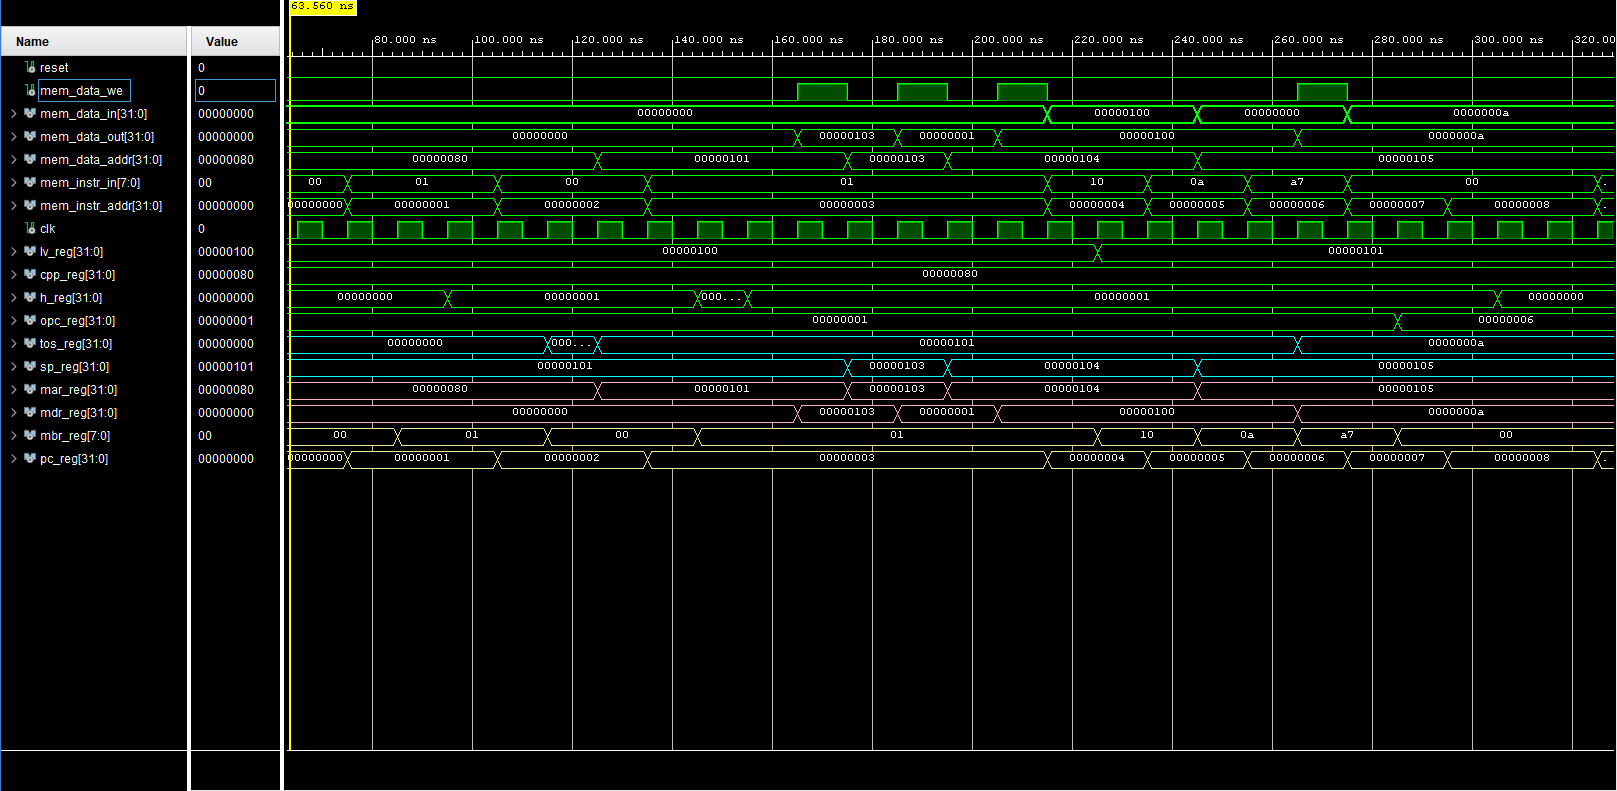
\includegraphics[width=17cm]{immagini/esercizio8/bipush_sim.png}
    \caption{Simulazione BIPUSH}
    \label{fig:bipush_sim}
\end{figure}

\subsubsection{Analisi IADD}
In questa sezione, si è scelto di esaminare il codice operativo IADD.
iadd = 0x65:
\begin{enumerate}
\item MAR = SP = SP - 1; rd: lettura del penultimo elemento dello stack.
\item H = TOS: salvataggio temporaneo di TOS in H
\item MDR = TOS = MDR+H: salvataggio in MDR e TOS della somma.

\end{enumerate}
Anche in questo codice operativo viene mostrato di seguito un esempio di rappresentazione binaria della prima microistruzione:
\begin{itemize}
    \item ADDR: 010011010
    \item JAM: 000
    \item Shift Register: 00
    \item ALU: 110110
    \item C: 000001001
    \item Mem: 010
    \item B: 0100
\end{itemize}

In Figura \ref{fig:bipush_sim}, è mostrato il risultato della simulazione quando viene eseguito il seguente programma:

\begin{lstlisting} [language=ant, caption=Programma simulazione IADD]
.main
.var
a
.endvar
BIPUSH 0xA
BIPUSH 0xE
IADD
ISTORE a
HALT
.endmethod
\end{lstlisting}



\begin{figure}[H]
    \centering
    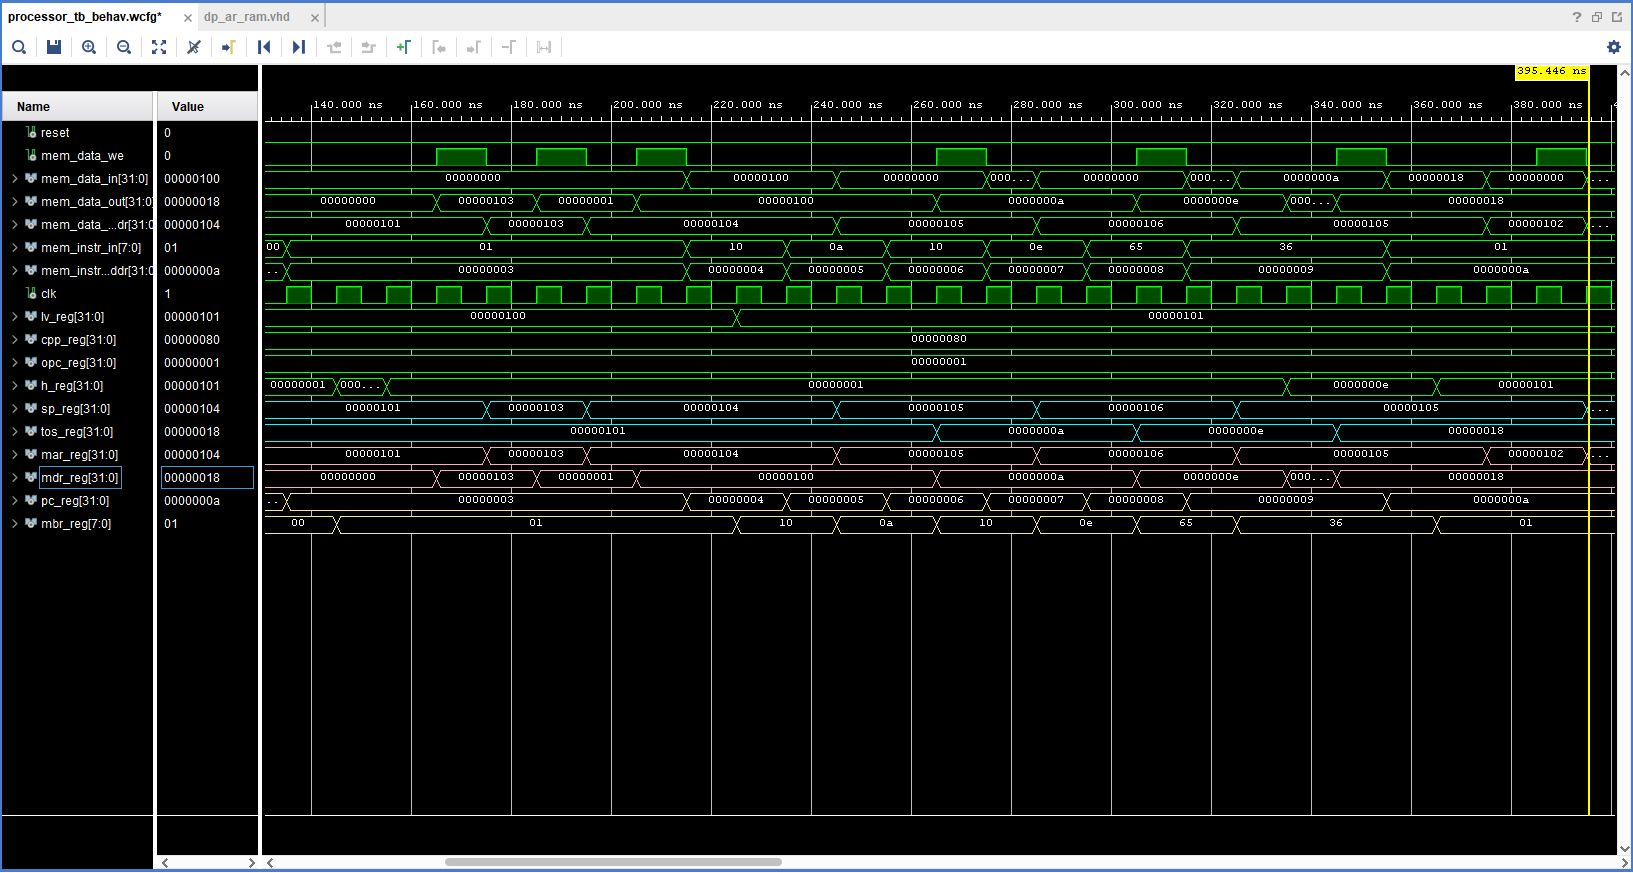
\includegraphics[width=17cm]{immagini/esercizio8/iadd_sim.png}
    \caption{Simulazione IADD}
    \label{fig:iadd_sim}
\end{figure}

\subsection{Modifica codice operativo IADD}
Per modificare il codice operativo sono stati innanzitutto installati i tool necessari a ricompilare le parti cambiate ovvero:\textit{Control Store}e \textit{la Memoria}. In particolare, è stato preso il codice operativo IADD ed è stata modificata la terza microistruzione: 

\begin{lstlisting} [language=ant, caption=Codice operativo IADD modificato in ISUB]
iadd = 0x65:
        MAR = SP = SP - 1; rd
        H = TOS
        MDR = TOS = MDR - H; wr; goto main
\end{lstlisting}

In questo modo invece di sommare \textit{H} a \textit{MDR} viene eseguita una sottrazione, infatti è possibile notare nel testbench qui riportato il nuovo valore del risultato in \textit{mem\_data\_out}:

\begin{figure}[H]
    \centering
    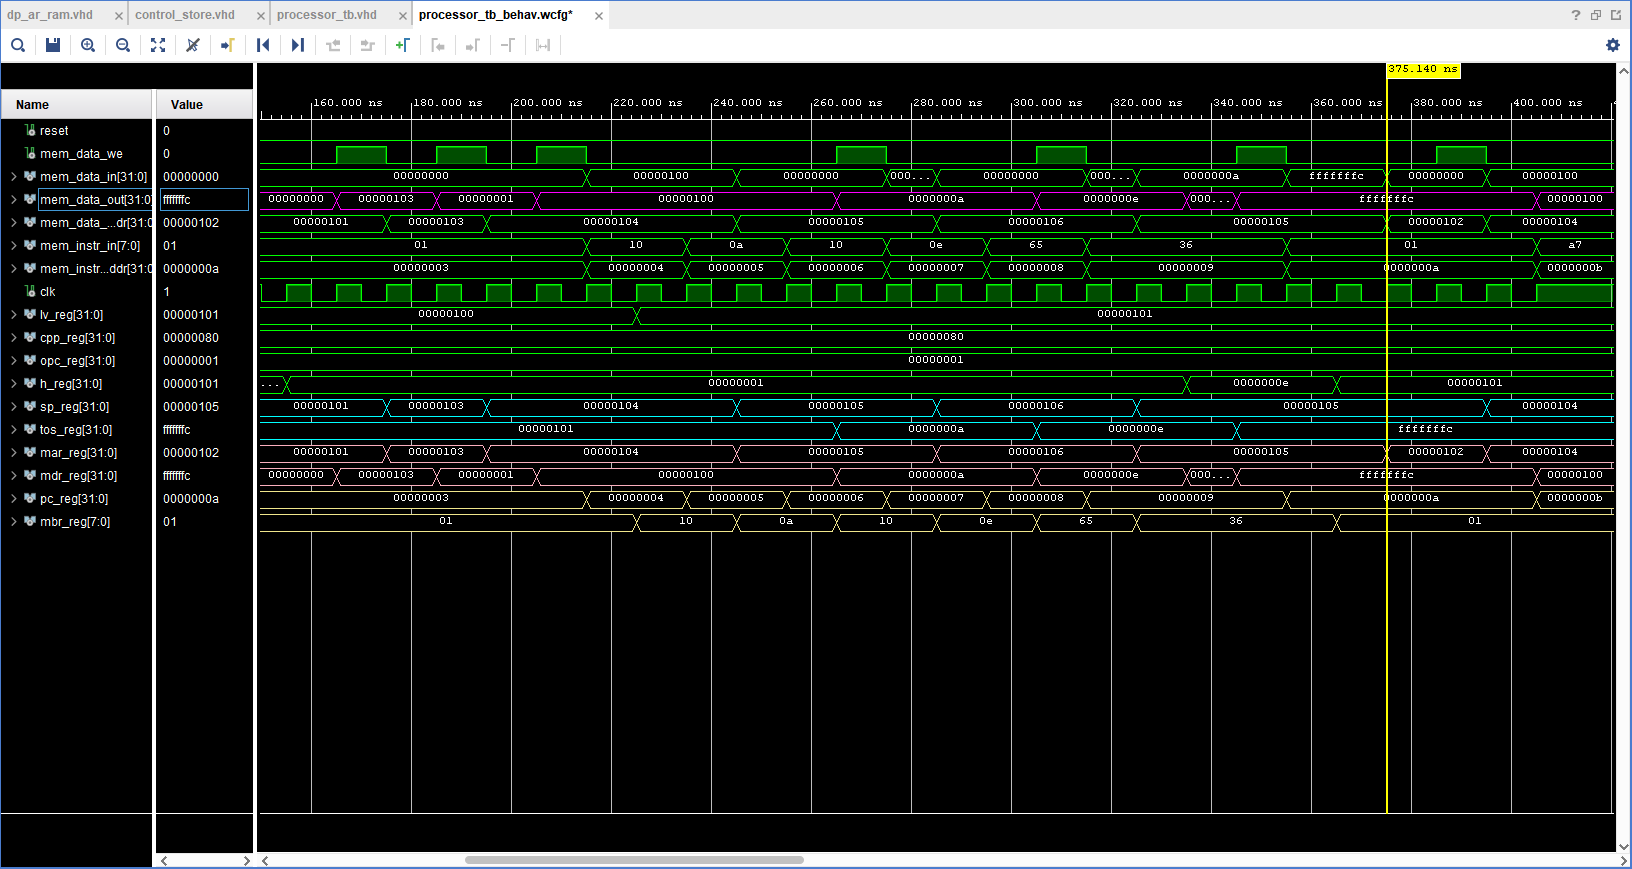
\includegraphics[width=17cm]{immagini/esercizio8/iadd_mod_sim.png}
    \caption{Simulazione IADD modificata in ISUB}
    \label{fig:iadd_imod}
\end{figure}



